\afterpage{\null\newpage}
\chapter{Adaptive Sampling Theory\label{ch:chapter3}}


In this Chapter, we investigate the theory of Adaptive Sampling with the goal to better understand the possibilities and limits of adaptive sampling. The results stated here were originally published in: 

\cite{Adstrategies2018} \textbf{Hruska, E.}; Abella, J. R.; N\"uske, F.;
Kavraki, L. E. \& Clementi, C.; Quantitative
comparison of adaptive sampling methods
for protein dynamics. J. Chem. Phys. 149 (2018) 

\section{Sampling Problem}

The stochastic behavior of biomolecules requires a good sampling of the process to understand the configurational behavior of the proteins accurately. This sampling can be done by molecular dynamics, and for small biomolecules such as peptides, this approach reaches a sufficient sampling. Larger biomolecules pose a significantly larger challenge to sample well. One cause are the slow collective motions that have long timescales. Figure~\ref{fig:raretransitions} illustrates that in many cases, there are rare transitions across a rare transition barrier. Simulating a longer molecular dynamics trajectory on one side of the barrier leads to a good sampling of one side of the barrier, but a low probability of crossing the rare transition barrier. This bottleneck causes an oversampling of the area on one side on the transition barrier.  

\begin{figure}[H]
  \centering
  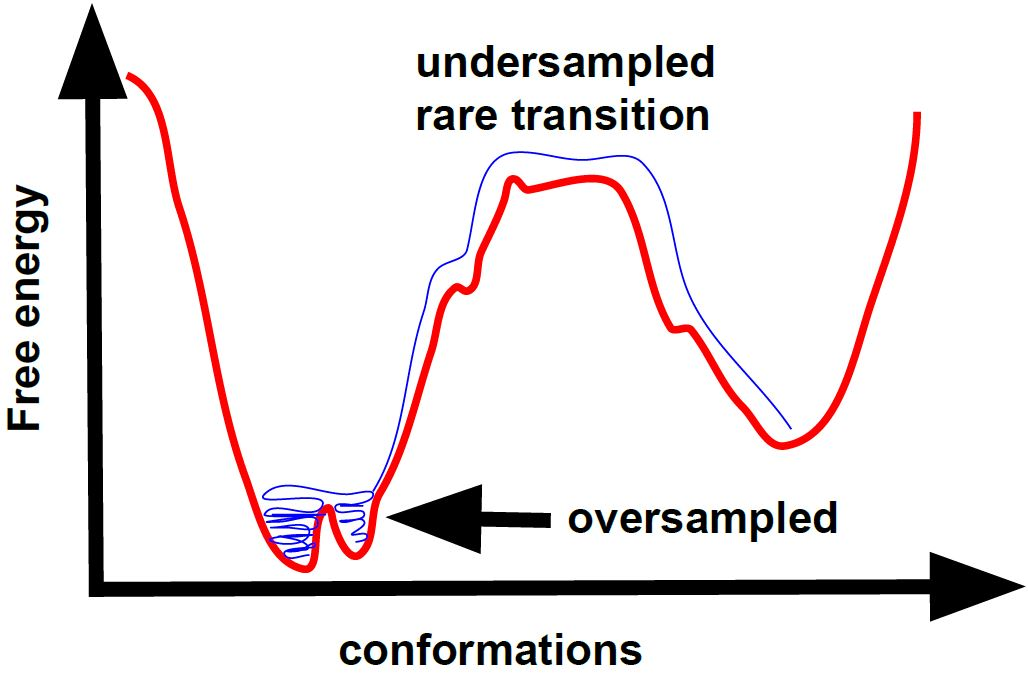
\includegraphics[width=0.9\linewidth]{figures3/rare_transition.pdf}
  \caption{Rare transitions barriers cause the sampling problem.}
  \label{fig:raretransitions}
\end{figure}

Figure~\ref{fig:raretransitions} shows the free energy landscape along on a reaction coordinate. The high sampling at the bottom of the free energy wells is caused by the Boltzman distribution, which describes the equilibrium probability density of configuration space for biomolecules. The equilibrium probability density $\pi$ is:

$$\pi(x)~e^{-F(x)/(k_{B}T)}$$

Here $F(x)$ is the free energy at reaction coordinate point $x$. The limited computational resources make long simulation times to sample the whole phase space of the biomolecules suboptimal. The computing power could be redirected to sample the rare transition barrier or the undersampled side of the transition barrier. For proteins, the rare transition barrier could be protein folding or other large-scale configurational changes.


\section{\label{sec:intro2}Alternative sampling approaches}

The sampling problem, as well the desire to accurately sample the dynamics of high-dimensional stochastic systems has led to many approaches besides adaptive sampling.
These efforts can be broadly categorized, but this summary can not exhaustively discuss all approaches due to a large number of these approaches.
One approach is to simulate longer molecular dynamics trajectories by software and hardware approaches. In recent years the utilization of Graphics processing units (GPUs) and the design of special-purpose hardware \cite{shaw2014anton}. The graphics cards can currently simulate almost 1 microsecond of MD trajectory per day of simulation time for smaller proteins. The Special purpose hardware can simulate up to 100 microseconds of MD trajectory per simulation day, but the major limitation of the special-purpose hardware is the minimal access to these machines. An important role also played software advances that can effectively utilize this hardware. Despite all the improvements, these approaches perform simple molecular dynamics simulations and don't utilize any additional possibilities of reaching longer timescales.

Another approach, incentivized by the increase in parallelization of High-Performance Computers, is the simulation of many simultaneous trajectories \cite{DistComp-Shirts2000, DistComp-Buch2010}. The sampling is performed in parallel for the same system, and by analyzing the resulting trajectories, a better sampled result is obtained.  As shown in Chapter 4, the total efficiency of sampling is reduced due to the independent nature of the sampling, but the absolute simulation time or the time to solution is reduced.

Monte Carlo is commonly used to improve the simulations of many stochastic systems. Here the sampling is not constrained to a hypersurface of conserved Hamiltonians, as is the case of molecular dynamics. This allows Monte Carlo to perform large jumps in configuration space, which is impossible in molecular dynamics. The high dimensionality of biomolecular systems reduces the effectivity of Monte Carlo Simulations, which doesn't represent well the collective motions of biomolecules. The approach of Hybrid Monte Carlo attempts to combine the strength of both Monte Carlo and MD, by including information of the intermolecular forces in the Monte Carlo moves. This approach is promising but wasn't yet able to reach longer timescales for biomolecules than other approaches. 


Modifying the Hamiltonian of the biomolecules is another common approach to solving the sampling problem. Here the Free energy barrier is reduced by adding terms to the original Hamiltonian of the biomolecules.
The reduced free energy barrier leads to shorter timescales necessary to sample the modified Hamiltonian. Different approaches such as metadynamics \cite{laio2008metadynamics} or accelerated MD\cite{hamelberg2004accelerated} are possible. The stationary probability distribution can be recovered according to the Boltzman distribution. Accurate kinetic information or conformational dynamics cannot be measured directly. Recent methods in recovering the kinetic information\cite{pathreweight1, pathreweight2, pathreweight3, pathreweight4} are investigated but haven't been widely used. 



\section{\label{sec:design}Adaptive sampling schema}


The general idea of \emph{adaptive sampling} \cite{singhal2005error, bowman2010enhanced,
weber2011characterization, Fabritiis-2014, preto2014fast, doerr2016htmd,
AdaptivePELE-Lecina2017, EvolutionCoupling-Shamsi2017, FAST-Bowman-2015, 
Strategies-erros-reduce, plattner2017complete, Adstrategies2018} is the ``divide and conquer`` approach. Simulating shorter molecular dynamics trajectories allows changing the restarting points for the next short molecular dynamics trajectories. The choice of this restarting points is a key element of this thesis. Figure~\ref{fig:branching} illustrates that the free choice of restarting points allows to clone configurations and sample certain areas of the energy landscape better. The black crosses in the figure indicate areas where sampling is blocked, reducing the utilization of computational resources in some areas.
Adaptive sampling allows the use of multiple parallel simulations and is therefore effective on High-Performance Computers (HPC).

\begin{figure}[h]
  \centering
  \includegraphics[width=0.6\linewidth]{figures3/branching_picture.pdf}
  \caption{Restarting method in adaptive sampling strategies.}
  \label{fig:branching}
\end{figure}


In the iterative process of adaptive sampling, the previously generated molecular dynamics trajectories are analyzed, and the analysis results inform the restarting points for the batch of
molecular dynamics trajectories. Figure~\ref{fig:schema2} shows the initialization and the 4 steps of adaptive sampling. Different adaptive sampling strategies have different implementation of the analysis steps, Steps 2 and 4. 

\begin{figure}[h]
  \centering
  \includegraphics[width=0.5\linewidth]{figures2/schema1.pdf}
  \caption{Basic schema of adaptive sampling. The
  number of starting conformations, analysis strategies or Step 3 stop condition are flexible and can be changed. Identical schema to Figure~\ref{fig:schema}.}
  \label{fig:schema2}
\end{figure}

The individual adaptive sampling steps are summarized as follows:
\begin{itemize}
\item Start: Initialization of the start configurations.  Commonly an unfolded structure of the selected proteins is chosen.
\item Step 1: Simulating an ensemble of MD trajectories. The configurations are chosen either by Initialization or Step 4. 
\item Step 2: Analysis of all previously generated MD trajectories. The analysis varies between adaptive sampling strategies.
\item Step 3: Stop condition. Automatic determination if the objective of adaptive sampling is achieved. When the objective is not achieved, proceed iteratively to Step 4. 
\item Step 4: Selection of restart configurations for the next set of MD trajectories based on the analysis results 
\end{itemize}

The beginning step of any adaptive sampling is the initialization. The start configuration from where adaptive sampling is launching is chosen. For each replica, which depends on the parallelization of the computational resource, a configuration is generated. The start configuration can be all identical or disparate. For proteins commonly an unfolded state is chosen.
In step 1, the MD simulations for all replicas are performed in a parallelized mode. Here most of the computational resources are utilized, and scalability of this step is crucial. Commonly  
Following the MD simulation is the analysis of the MD trajectories in step 2. In the following Chapters 5 and 6, the adaptive sampling strategies $cmicro$ and $cmacro$ with Markov State Models \cite{prinz2011markov} are used as described in this Chapter. 

The results of Step 2 allow determining in Step 3 if the objectives of adaptive sampling are reached. Examples for the objectives are protein folding, achieving a certain accuracy in protein dynamics, or exploration of a part of the energy landscape corresponding to a smaller-scale motion of the protein. If the objective is not reached, Step 4 creates the restarting configuration for the next MD trajectories corresponding to Step 1. The adaptive sampling strategies to determine the restarting points in Step 4 in Figure~\ref{fig:schema2} are easily exchangeable, such as the strategies discussed below. Once the objective in Step 3 is reached, adaptive sampling finishes and all trajectories can be further analyzed. Here usually, the dimension reduction and analysis methods used for restarting are utilized to obtain accurate stationary and dynamics information about the biomolecule.


\section{\label{sec:intro2}Adaptive sampling strategies}
The general advantage of adaptive sampling compared to other non-adaptive sampling strategies is the resulting accurate conformation dynamics results and improved timescales reachable. While the success of adaptive sampling has been demonstrated in applications \cite{Wieczorek2016,Plattner20171005,Kohlhoff201415}, the success of adaptive sampling depends on the chosen adaptive sampling strategy. Different methods have been proposed and investigated\cite{Fabritiis-2014,
AdaptivePELE-Lecina2017, preto2014fast, doerr2016htmd,
weexplore, prattWESTPAAdvancesSampling2018, Adstrategies2018, FUNN, FAST, harada2015jctc, singhal2005error, bowman2010enhanced,
weber2011characterization,  EvolutionCoupling-Shamsi2017, FAST-Bowman-2015, 
Strategies-erros-reduce, plattner2017complete, WESTPA-Zwier2015}. 

Despite the range of adaptive sampling methods, there is no consensus which adaptive sampling strategies perform best for which sampling goal. This lack of comparability between different adaptive sampling strategies is partially caused by the number of disparate ways the individual adaptive sampling methods are implemented. In Chapter 5, a flexible software framework is developed, which allows the utilization of any of the adaptive sampling strategies and improves the comparability between the adaptive sampling strategies.

One common difference between the adaptive sampling strategies is the method to dimension reduce the molecular dynamics trajectories. The dimension reduced molecular dynamics trajectories are generally easier to analyze further.
Some adaptive sampling strategies such as CoCo-MD\cite{shkurti2019jctc,harada2015jctc,harada2017jctc} use PCA. Other dimension reduction methods are TICA\cite{TICA1-perez2013, TICA2-schwantes2013}
, Diffusion Maps \cite{Coifman7426, rohrdanz2011determination,Zheng2011, Boninsegna2015},
likelihood-based approaches \cite{peters2006obtaining}, cut-based free energy
profiles \cite{krivov2008diffusive}, or neural networks such as VAMPnets (SRV)
\cite{Mardt2018,wehmeyer2018time, ribeiro2018reweighted, chen2019jcp}. 

Multiple layers of dimension reduction such as combining TICA with Markov State Models (MSMs) \cite{prinz2011markov,
MSM-Pande-2018,bookmsm,masterequationsMSM,SCHUTTE1999146} are common. MSMs are able to process many short trajectories and
do not require equilibrium sampling to recover thermodynamics and kinetic properties. The ability of non-equilibrium sampling is essential for adaptive sampling.
The most common dimension reduction methods are TICA in combination with Markov State Models (MSMs) due to the validation of this approach, but new approaches such as VAMPnets offer some benefits such as the ability to analyze shorter trajectories at same accuracy. Shorter trajectories allow potentially a more frequent restarting for adaptive sampling.

The restarting strategies based on the dimension reduced trajectories show significant variety, making a comparison complex.

Some of the common restarting strategies are the $cmicro$ and $cmacro$ strategy, and adaptive sampling with \emph{a priori} information. These strategies are described in the following section. 

\section{\label{sec:restart-strategies}Restart Strategies for Adaptive Sampling}


Different adaptive sampling strategies can be broadly categorized into strategies with and without \emph{a priori} information. In the following section, the adaptive sampling strategies $cmicro$ and several types of $cmacro$ are introduced, which all don't utilize \emph{a priori} information. These strategies select restarting positions only according to the iteratively updated analysis results. 

To contrast two two strategies utilizing \emph{a priori} information, $Q_{f}$ and $Q_{f,nn}$, are introduced. These strategies take advantage of the previously known slow collective modes for the studied protein or utilize the intuition of the domain experts on the behavior of proteins. The introduced strategies are not exhaustive but cover the more commonly used adaptive sampling strategies. 

Common to these strategies is the use of MSM for the analysis, due to the effective analysis of the non-equilibrium trajectories generated by adaptive sampling. Chapter 2 described the steps standard in generating an MSM from the adaptive sampling. The MSM is repeatedly generated for each iteration of the adaptive sampling to include the additional molecular dynamics trajectories. 

\subsection{Adaptive sampling strategy $cmicro$}
One less complex adaptive sampling strategy is the $cmicro$ strategy, also called $1/C$ strategy. This strategy chooses the restart
states on the count of molecular dynamics trajectories that have visited each MSM state \cite{weber2011characterization, Fabritiis-2014, AdaptivePELE-Lecina2017,doerr2016htmd}.
By restarting in less visited states, the undersampled areas of the proteins will be sampled more. Generally, for a given MSM state $i$, the restart probability is proportional inversely to count for this state. The c in $cmicro$ strategy stands for the count of times molecular dynamics trajectories have each state. The $cmicro$ strategy is particularly effective in exploring, but less effective in crossing rare transition regions \cite{Adstrategies2018}.


\subsection{\label{sec:macro}Adaptive sampling strategy $cmacro$} 
A further development of the $cmicro$ strategy is the v, also called $1/C_M$ strategy.
To improve the crossing of rare transition regions, additional kinetic information of the MSM states is taken into account. 
A higher restart probability is chosen for states which are kinetically disconnected. This is implemented by clustering the MSM into kinetically connected states. Two clustering methods can be used, 
PCCA+ \cite{roblitz2013fuzzy}, or k-means clustering of the MSM in the MSM eigenvector dimensions \cite{preto2014fast, doerr2016htmd}. Each of the resulting clusters is one macrostate.
Any MSM states not connected in the MSM is treated as an additional macrostate. 
The restarting probability is proportional to $1/C_{macro})$, where $C_{macro}$ is the count of molecular dynamics trajectories have visited each macrostate. From each restart macrostate, the restart states are selected inversely proportional to the state count.
In this work, we investigated the effects of 4 variants of the $cmacro$ strategy. One difference is the approach to setting the number of macrostates. The number of macrostates affects the kinetically connected states and affects the effectivity of this adaptive sampling strategy. 
One approach is to set the number of macrostates to a constant number such as 30. The other approach is to determine the number of macrostates based on the number of
slow collective motions of the protein, here the number of dimensions with collectively have 50\% of the total kinetic content of the system. 

An additional variation of the $cmacro$ strategy is designed to reduce the effect of the non-equilibrium data on adaptive sampling. In the first step of the analysis, the dimension reduction of the molecular dynamics trajectories is affected by the non-equilibrium sampling of the trajectories. This non-equilibrium sampling is caused the different restarting probabilities across the protein landscape. One approach to reduce the effect of this non-equilibrium sampling on the dimension reduction is the Koopman reweighting method
\cite{koopmanold, koopman2,koopman3,koopman4, wu2017variational, Nueske2017}. Here first, the stationary distribution is estimated, and then this stationary distribution is utilized to reweight the input molecular dynamics trajectories towards the stationary distribution. For adaptive sampling, the estimate of stationary distribution will only be partially correct due to only partially sampling the whole protein energy landscape. The improvement in dimension reduction leads to an improved MSM and better restarting probabilities. 

The 4 variants of the $cmacro$ strategy are the following:
\begin{description}
\item[$1/C_{M,1}^C$]
The MSM is not adjusted, and the number of macrostates is fixed at 30.
\item[$1/C_{M,2}^C$]
The MSM is not adjusted, and the number of macrostates is based on the number of timescales with a 50\% kinetic content.
\item[$1/C_{M,1}^K$]
The MSM is corrected to represent the equilibrium MSM, and the number of macrostates is fixed at 30.
\item[$1/C_{M,2}^K$]
The MSM is corrected to represent the equilibrium MSM, and the number of macrostates is based on the number of timescales with a 50\% kinetic content.
\end{description}

The effectivity of setting of the number of macrostates based on the number of timescales depends on the individual proteins and sampling of the protein behavior.
For this reason, the more robust approach of using a constant number of macrostate together with the Koopman correction $1/C_{M,1}^K$ is used as the default variation of the $cmacro$ strategy.
All 4 variants have the goal of crossing slow transition barriers faster of folding proteins faster \cite{Adstrategies2018}.


\subsection{Adaptive sampling with \emph{a priori} information}

\emph{A priori} information about the protein can significantly speedup the adaptive sampling by guiding the direction in which to sample. One approach \cite{EvolutionCoupling-Shamsi2017} proposed restarting based on the number of folded contacts based on the evolutionary coupling analysis. The FAST method \cite{FAST-Bowman-2015} utilizes the distance to a target structure. The effectivity of this approach also depends on the quality of the \emph{a priori} information. This general class of adaptive sampling strategies will be studied in this work by two different strategies, $Q_{f}$  and $Q_{f,nn}$.  

\subsubsection{Adaptive sampling strategy $Q_{f}$}

The  $Q_{f}$ adaptive sampling strategy utilizes the native contacts to guide the sampling. Using the \emph{a priori} known folded structure of the protein, for each state $i$, the number of native contacts $Q_i$ is calculated. To adaptively sample the folded state from the unfolded state, states with a higher number of native contacts are preferred. The restarting probability is proportional to $exp( - k * | Q_i - Q_{max} | )$. Here, $Q_{max}$ is the total number of native contacts. The parameter $k$ controls the strength of guidance by this reaction coordinate and is in the range of 0.1 and 1, with a smaller number generally for larger proteins. This strategy works effectively when the folding path of the protein is simple. For some proteins, this strategy leads to misfolded states with high $Q_i$. Return to the folding path is slow with this strategy since some contacts would have to be broken, which corresponds with a low restarting probability.

\subsection{Adaptive sampling strategy $Q_{f,nn}$}

The strategy $Q_{f, nn}$ is designed to prevent the misfolded states from strategy $Q_{f}$.
Here both native and non-native contacts are utilized in calculating the restarting probabilities. Restarting in states with a higher number of non-native contacts is reduced.
The restarting probability in state $i$ is proportional to $exp(-d_i)$, where $d_i = \sqrt{k_1^2 * (Q_i - Q_{max})^2  + k_2^2 * N_i^2}$. 
The additional parameters to strategy $Q_{f}$ are $N_i$, which is the number of
non-native contacts, and $k_1, k_2$ are setting the strength of the sampling pressure along the native and non-native contact dimensions. This strategy avoids misfolded states and is faster and more robust than $Q_{f}$.

\subsubsection{Additional restarting strategies}
Some additional restarting strategies are the following:
DeepDriveMD\cite{leeDeepDriveMDDeepLearningDriven2019} restarts from outlier points detected by the Density-based spatial clustering methods DBSCAN. This approach depends on the effectivity of the dimension reduction of the molecular dynamics trajectories. CoCo-MD extrapolates the restarting points outside of the already sampled configurations based on PCA projection\cite{shkurti2019jctc,harada2015jctc,harada2017jctc}.  

All these adaptive sampling restart strategies have similar, but not identical goals.
Some of these goals are the faster crossing of rare transition barriers, such as protein folding, of accurate configurational dynamics results, or sampling of a small part of the energy landscape.
The effectiveness of the individual adaptive sampling strategies for each of these goals is, in many cases, unclear. Studies \cite{preto2014fast,weber2011characterization,bowman2010enhanced,Fabritiis-2014} report speedup of protein folding with adaptive sampling between 2 and 10, but in most cases, these studies have small sample size. Chapter 4 evaluates some of the adaptive sampling strategies for two different goals: crossing a rare transition barrier, such as the folding of a protein and the speedup of the exploration of large regions of the conformational space of a protein.

\subsection{plain MD} 

While plain MD is not an adaptive sampling strategy, it is used as a comparison for all the adaptive sampling results. To illustrate the main difference with adaptive sampling, for plain MD no analysis is performed after each iteration, Steps 2 and 4 are missing. Instead, each MD trajectory is continued in the next iteration. To allow comparison with adaptive sampling, the parallelization of plain MD is chosen to be equal to the parallelization of adaptive sampling.  

\section{Upper limits to adaptive sampling strategies}

\subsection{Optimal strategy for exploration: $p_{esc}$}

One objective for adaptive sampling is the optimal exploration of all states. This objective is relevant when the whole energy landscape has to be explored with no dominant slow processes. 
An upper limit can be derived when assuming that the full transition matrix for the protein investigated is known. The full transition matrix is not generally known and limits this strategy only as an upper limit speed of exploration. No adaptive sampling strategy can explore all the states faster. This approach assumes that the transition matrix represents the protein accurately.
First, we calculate for each visited microstate $i$ the probability of transition to any microstate, which is not explored yet.

$$p_{esc}[i]=\sum_{j \in unexplored}T[i, j]$$

For this optimal strategy, the next restarting configuration is chosen from the state with the highest $p_{esc}$. The performance of this upper limit on exploration speed is investigated in Chapter 4.

\subsection{Optimal strategy for protein folding: $t_{opt}$} 

Many biomolecules have significant transition barriers, which cause slow collective motions. Here the objective is to cross the transition barrier optimally.
The problem can be rephrased as the mean optimal time to reach any state in the ensemble  $s_1$. Frequently this ensemble of states is the folded state.  
Similarly to the $p_{esc}$ strategy we assume the full transition matrix for the protein is known. As the first step we designate the mean optimal time to reach $s_1$ from state $i$ as $t_{opt}[i]$.
For every state in $s_1$ the value of  $t_{opt}[i]$ is zero.

All these $t_{opt}[i]$ values have interdependencies caused by our knowledge of the full transition matrix:

$$t_{opt}[i]=\sum_{j \in states}T[i,j]min(t_{opt}[i],t_{opt}[j])+1$$

This equation has two parts. The first part represents the restarting of the adaptive sampling in the current state $i$. According to the transition probability, the next steps would be state $j$. The new state $j$ is only accepted if the mean optimal time of state $j$ is lower than the current state. All previously explored states with higher $t_{opt}$ are insignificant since the optimal strategy chooses only the state with mean optimal time. The addition of 1 is caused by the one restarting iteration in the first part. The result is in units of restarting steps. The above equation can be solved numerically. The performance of this strategy $t_{opt}$ defining the upper limit on folding speed is investigated in Chapter 4.

We then use it to define a benchmark restart strategy by
selecting the restart state among the ones explored that has the lowest
$t_{opt}$ value, representing the state that is the closest to the folded
state. Note again that this strategy is impossible to implement in
practice, but still is a useful benchmark for adaptive sampling strategies.
With the $t_{opt}$ benchmark the maximum achievable speedup with adaptive
sampling for the folding of a protein can be evaluated.


\section{\label{sec:methods}Discussion}

The two new upper limits on adaptive sampling speedup allow for an increased understanding of adaptive sampling strategies, continued in Chapter 4. Without any theoretical upper limit, the potential of adaptive sampling is unknown. The equations show that the potential of adaptive sampling depends on the transition matrix, which changes with each protein. Adaptive sampling strategies will be more effective when following the restarting decisions of $t_{opt}$ benchmark under the constrain of no \emph{a priori} knowledge of the transition probabilities.



















